\section{Architecture}
\label{sec:architecture}
\system{} is an extension of \moodle{} and can be seen as a package of plugins. 
The architecture does not specify how each plugins should be created, but specifies a general structuring of the components of the system. 
The complete architecture can be seen in \figref{fig:architecture}.
\begin{figure}[h!t]
	\centering
		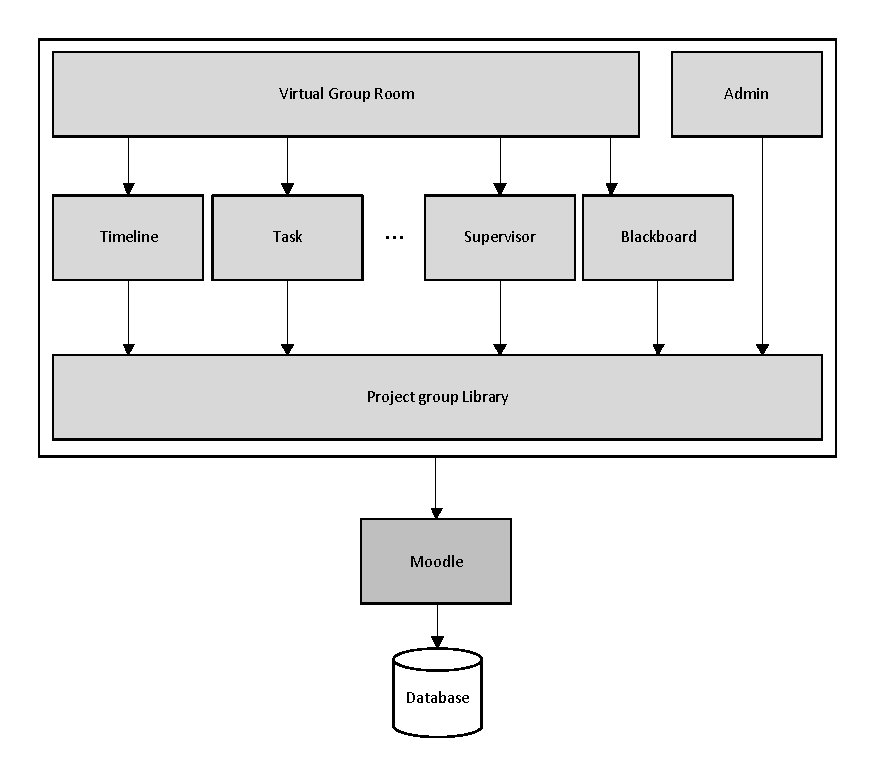
\includegraphics{images/architecture.pdf}
	\morscaption{The overall architecture of MyMoodle}
	\label{fig:architecture}
\end{figure}

The system architecture consists of a total of five layers. 
The three uppermost constitute \system{}, they have a common dependency, namely the Moodle platform. 
Layers four and five are Moodle and the Database respectively.
%Our extension  as a plugin of Moodle and use functions supplied by Moodle to function.

We explain the three uppermost layers as:
\begin{enumerate}
	\item The uppermost layer is the project group view and the administration tool.
	The project group view is used for presenting the virtual meeting place for a project group.
	It is described in \secref{sec:virtualMeetingPlace}.
	The administrative tool is a tool used by administrative personnel for managing project groups.
	It is described in \secref{sec:groupManagement}.
	This layer is called ``View Layer''.
	\item Directly below the upper most layer is the ``middle'' layer which consists of the four parts: Timeline, Task, Supervisor, and Blackboard.
	These four parts are created by our peer-groups and are not explained further.
	We call this layer ``Content Layer'' since the components in this layer generate content for the Project Group View component.
	\item Below the middle layer is the project group library which contains common functionality.
	This layer handles all intercommunication between the parts in the Content Layer.  
\end{enumerate}


There are two primary factors to be considered when planning an architecture. 
First, we are four sub-groups working together. 
This creates the need for a structured way of communicating between the different parts and it lets every \subgroup{} know how their part is connected to the rest of the project. 
Second, the project should be passed on, which requires an architecture that increases the comprehensibility of the project.
%alex -> <@:-D-|-<

It is not possible to make a strict layered architecture due to the Moodle dependency and the administrative tool, which does not have to use the intermediate layer, but depends directly on the project group library and \moodle{}.
We do, however, prohibit ourselves from accessing the database directly, by using the Moodle Database Layer (note that it is not a layer in our architecture) described in \secref{sec:moodleoplatformdbml}.
In \figref{fig:architecture} the dependency from the box encircling \system{} indicates that every component in \system{} depends on the \moodle{} component.
The \moodle{} component consists of the Database Layer as well as the Context System, Capabilities, etc.

%These considerations leads us to design the illustrated architecture in \figref{fig:architecture}.
Note that the relative size of the components do not imply anything, e.g.\ the Moodle component is much larger, code wise, than all of the components in \system{} combined, but is illustrated with a rectangle the same size as any of the Content Layer components.













